\documentclass{article}
\usepackage{graphicx} % Required for inserting images

\title{Hierarchical Large Language Models for Multi-task problems}
\author{simen }
\date{November 2023}

\usepackage[
backend=biber,
style=alphabetic,
sorting=ynt
]{biblatex}
\usepackage{amsmath}
\usepackage{booktabs}
\addbibresource{references.bib}

\begin{document}

\maketitle

\section{Introduction}
Large Language Models (LLM) have become a popular tool for solving a wide range of text problems. LLMs are typically pretrained on a large and diverse dataset, and then fine-tuned on a specific task. The fine-tuning process is often done by minimizing the negative log-likelihood of the task-specific dataset, and the resulting model is then used to make predictions on new data. A popular fine-tuning method is Low-Rank Adaption (LoRA), which reduces the number of trainable parameters by 10'000 times and the GPU memory requirement by 3 times, while still outperforming other fine-tuning techniques (\cite{hu_lora_2021}).

This paper presents a generalization of the LoRA fine-tuning method for multi-task problems, which we refer to as Hierarchical LoRA. The Hierarchical LoRA method allows tasks to share information between each other through a global parameter set, and can be seen as a generalization of the two conventional approaches for multi-task problems: (1) finetuning each task separately, and (2) training one model for all tasks. We evaluate the Hierarchical LoRA method on a benchmark dataset, and show that there exist a trade-off between the global and task-specific parameters that can be tuned to optimize the model's performance.

\begin{itemize}
    \item Typically one finetune each task separately, as written in \ref{eq:lik}.
    \item If the D tasks are more similar to eachother than the pretraining corpus, the optimal parameters $\hat{\theta}_d$ should share some information during training in order to maximize their likelihood.
\end{itemize}

\section{Related works}

\subsection{Low-Rank Adaption of Language Models}
Low-Rank Adaption (LoRA)

[This might be background?]
\begin{itemize}
    \item explain what pretraining LLM means
    \item Explain how LORA fine tuned is done on each task
    \item Explain how LORA finetuned also could be done on all tasks together if they have a similar data distribution.
\end{itemize}

\section{Method: Hierarchical LLM}


\subsection{Task and Data Structure}
We define our study across $D$ distinct tasks, denoted as $d=1,2,...,D$. For each task $d$, we have a dataset $\mathcal{D}_d$ containing $N_d$ documents, with each document consisting of a sequence of $W_n$ tokens. This dataset structure can be formally represented as:

\begin{equation} \label{eq:data}
\mathcal{D} = \{ \mathcal{D}_d \}_{d=1}^D  =  \{ \{ w_{d,n,1:W_n} \}_{n=1}^{N_d} \}_{d=1}^D
\end{equation}
%
In this notation, $w_{d,n,1:W_n}$ represents the token sequence in the $n^{th}$ document of the $d^{th}$ task. For simplification in subsequent discussions, we will omit the indices $d$ and $n$ when their reference is evident from the context.

\subsection{Pretrained Autoregressive Language Model}
Our foundational model is a pretrained autoregressive language model, denoted by its parameters $\theta_{full}$ and its architecture, referred to as $LLM$. The model's probability distribution is given by:

\begin{equation} \label{eq:LLMprob}
P(w_{1:W} | \theta_{full}) = \prod_{i=1}^{W-1} LLM(w_{i+1} | w_{1:i})
\end{equation}
%
Here, $\theta_{full}$ represents the set of parameters obtained from pretraining on a large and diverse dataset, distinct from our current dataset $\mathcal{D}$.
We omit to write $\theta_{full}$ explicitly in the model, as the autoregressive language model always depend on these parameters.

\subsection{The Hierarchical LoRA model}
For each task $d$ we have a LORA parameter set $\theta_d$ that is used to fine-tune to that task.
Hence, the likelihood of our problem follows from combining equation \ref{eq:data} and \ref{eq:LLMprob}:
\begin{equation} \label{eq:lik}
    \text{L}(\mathcal{D} | \theta_1, \theta_2, \ldots, \theta_D) = \prod_{d=1}^D L(\mathcal{D}_d | \theta_d) = \prod_{d=1}^D \prod_{n=1}^{N_d} \prod_{i=1}^{W_n-1} \text{LLM}(w_{d,n,i+1} | w_{d,n,1:i}; \theta_d)
\end{equation}
%
%
Each task will share some information with each other, and we model this by introducing a Gaussian hierarchical prior over the task parameters $\theta_{1:D}$, given by
\begin{equation} \label{eq:prior}
    P(\theta_{1:D} | \Theta, \tau ) = \prod_{d=1}^D N(\theta_d ; \Theta, \frac{1}{\tau} I)
\end{equation}
%
where $\Theta$ is a set of hierarchical mean parameters, $I$ is a unit diagonal matrix and $\tau \geq 0$ is a scalar precision hyperparameter controlling how similar task parameters $\theta_d$ should be to the hierarchical mean parameters $\Theta$.
We let $\Theta$ have a uniform prior (i.e. $P(\Theta) = 1$).

The posterior distribution of the hierarchical model is then given by combining equation \ref{eq:lik} and \ref{eq:prior}:
\begin{equation} \label{eq:posterior}
    P(\theta_{1:D} | \mathcal{D}, \tau) \propto \prod_{d=1}^D \text{L}(\mathcal{D}_d | \theta_d) \cdot P(\theta_d | \Theta, \tau)
\end{equation}
%

\subsection{Optimization}
Given a precision hyperparameter, we want to find the maximum a posteriori (MAP) estimate of the hierarchical model. We will do this by using AdamW (\cite{adamW}), a gradient-based optimization algorithm, optimizing over the task parameters $\theta_{1:D}$ and the hierarchical mean parameters $\Theta$ simultaneously.

\section{Experimental setup}
% Use the Talk of Norway Dataset consisting of speeches of Norwegian parliament politicians. We will consider different speakers of this dataset as different tasks, and see how the hierarchical model can benefit from sharing information between these tasks.

% As base model, use opt-350m as it is predominantly trained on English, and only has seen a small amount of Norwegian data from the commoncrawls dataset.
To test our method, we optimize the model with a range of different precision hyperparameters $\tau$, and evaluate the model's perplexity on the test set for each task.


We use the Talk of Norway Dataset \cite{lapponi_talk_2018}, which consists of speeches of Norwegian parliament politicians. Each speaker will come from different political parties and geographical areas, but the tasks will still share a common domain. Therefore, we can consider different speakers of this dataset as different tasks. Specifically, we select chronologically the 25 first speakers that have above 100 speeches in the dataset.
This gives us a total of 25 tasks with samples ranging from 110 to 477 documents, and an average of 202 documents per task.
The distibution of samples per task can be seen in Figure \ref{fig:task_len}.
We split the training and test datasets randomly for each task in a 67/33 ratio.

% add figure of the dataset distribution in file training_lengths.png
\begin{figure}[h] \label{fig:task_len}
    \centering
    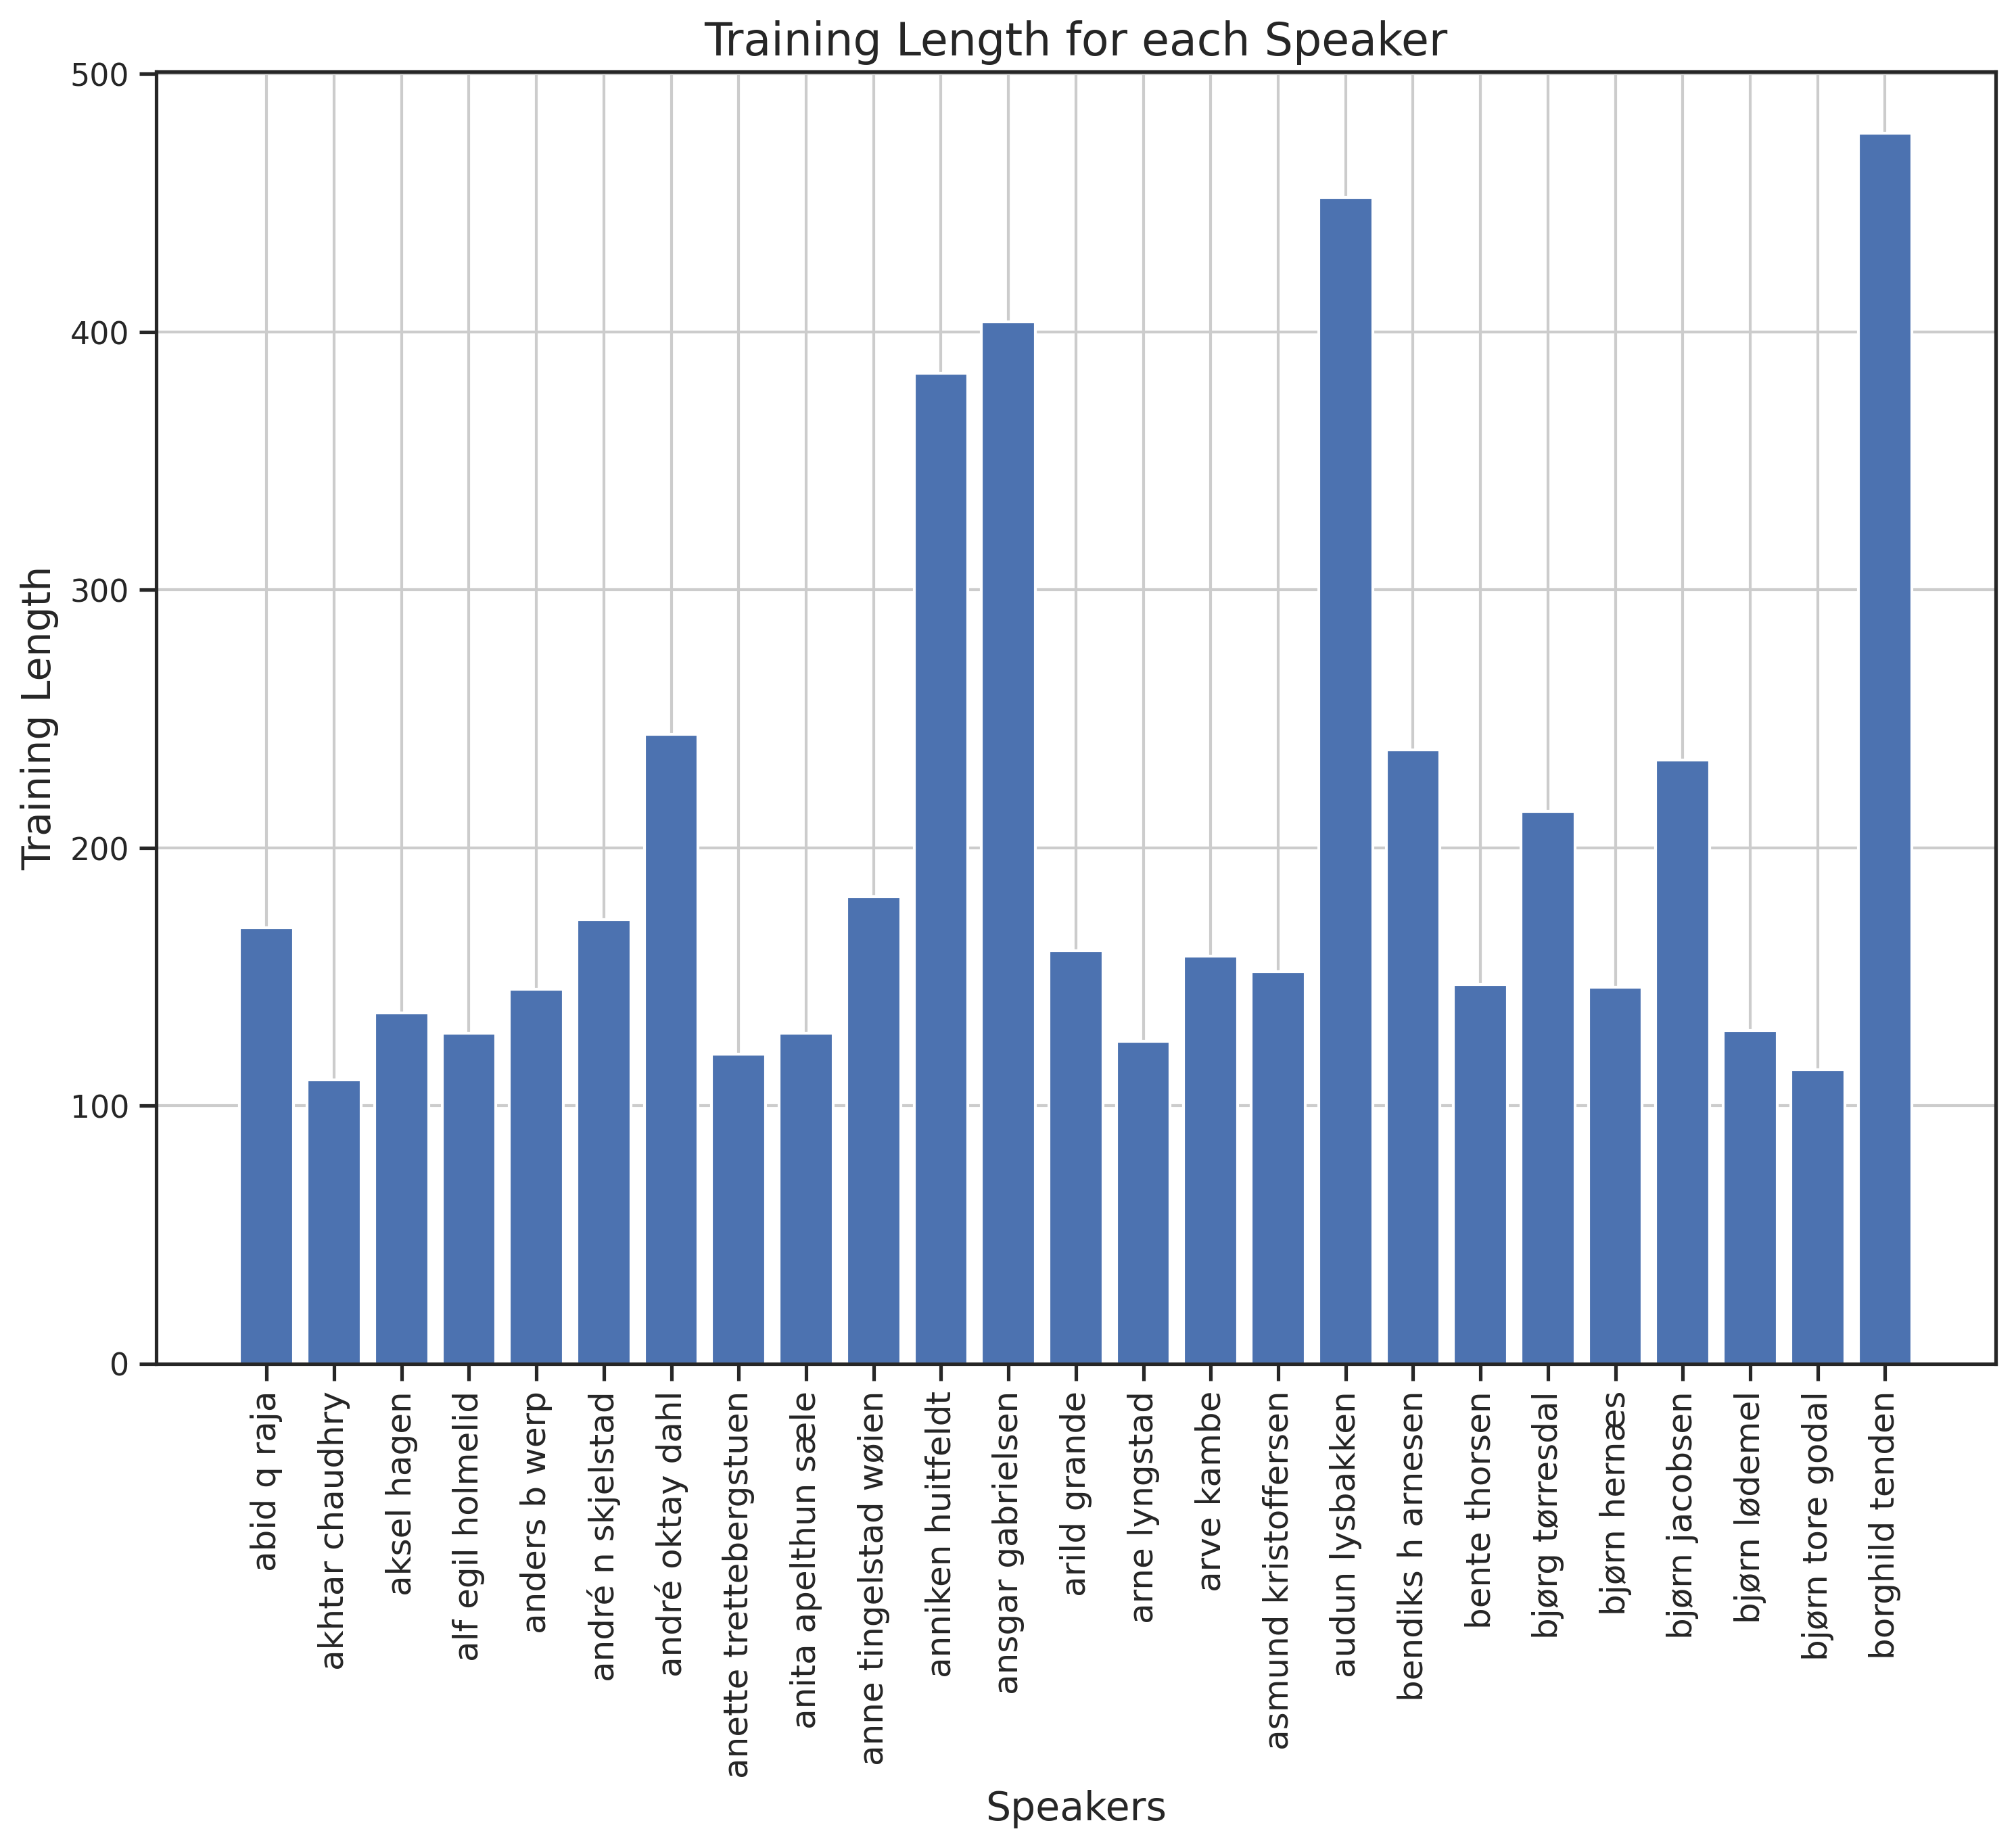
\includegraphics[width=\textwidth]{figures/training_lengths.png}
    \caption{Number of training examples for each task}
    \label{fig:training_lengths}
\end{figure}

We select a model that has been pretrained on a large and diverse dataset, but has not seen the specific tasks that we want to evaluate it on. We will use the `opt-350m` model \cite{zhang_opt_2022}, which is predominantly trained on English, and has only seen a small amount of Norwegian data from the CommonCrawls dataset.

Adapting learning rate to the precision hyperparameter..

\section{Results}

\begin{figure}[h]
    \centering
    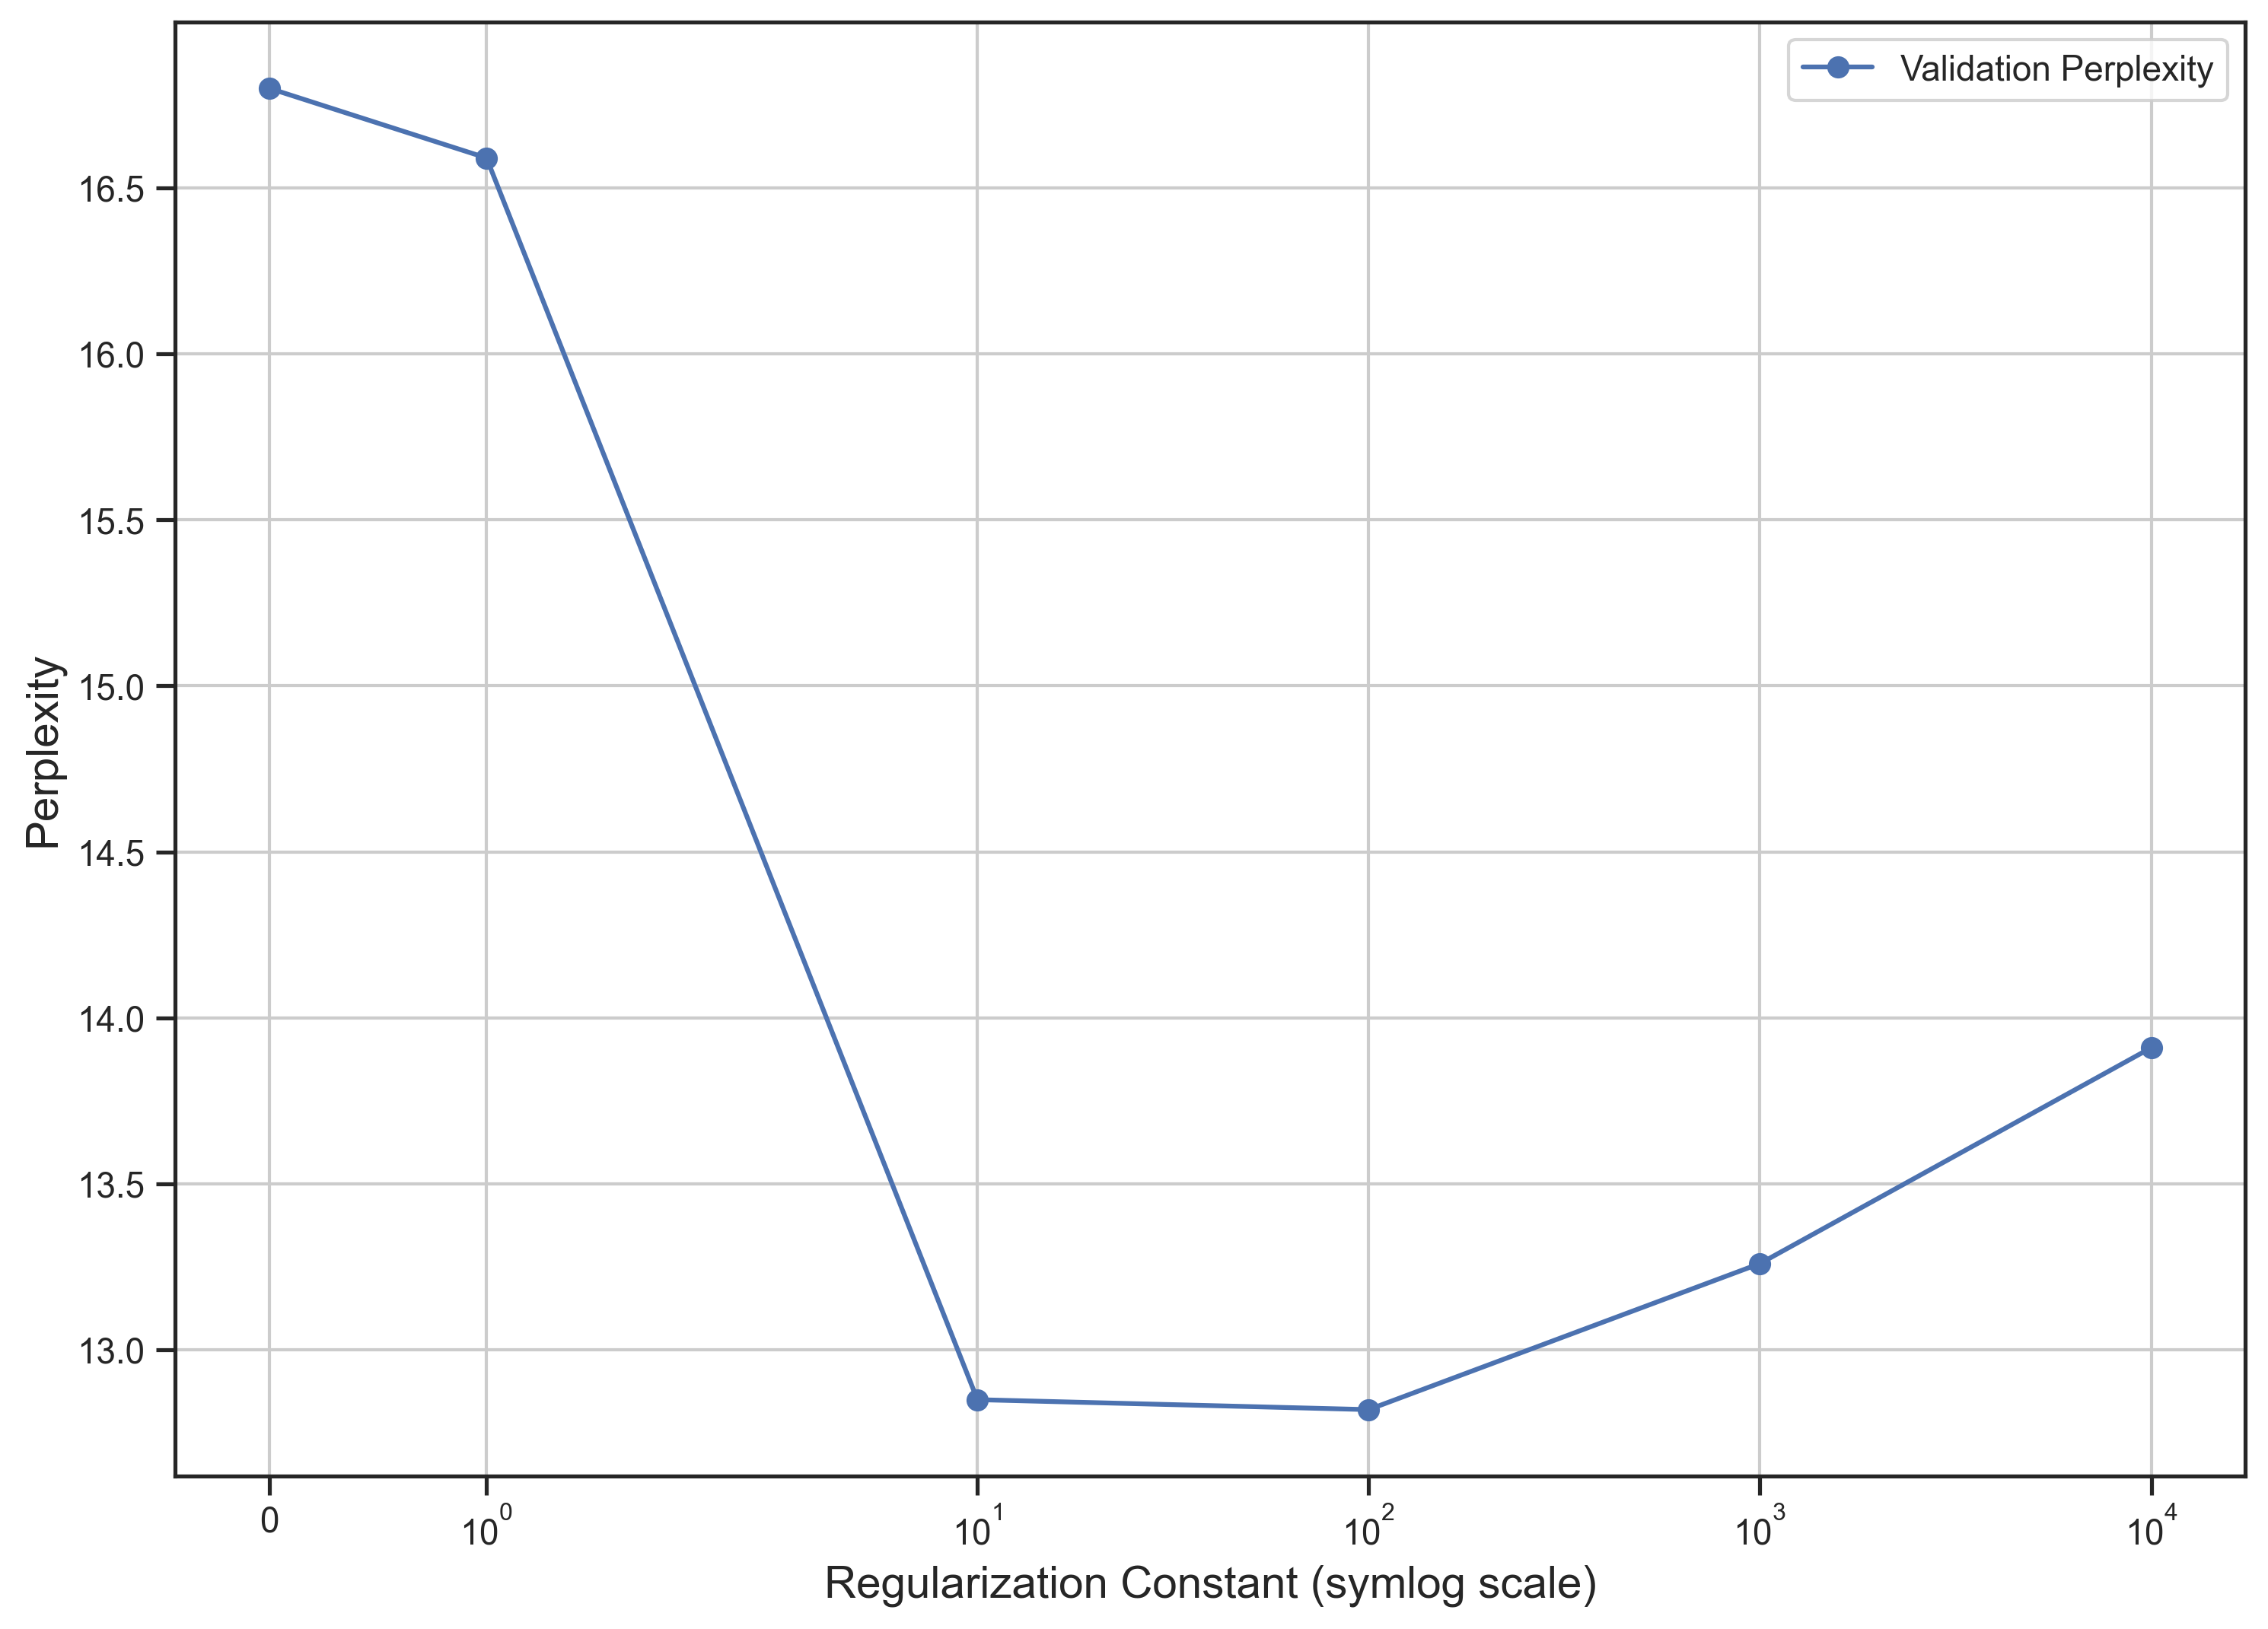
\includegraphics[width=\textwidth]{figures/results_plot.png}
    \caption{Plot of Regularization Constant vs Perplexity}
    \label{fig:results_plot}
\end{figure}

\begin{table}[h]
\centering
\caption{Empirical results of the hierarchical LORA finetuned on the three tasks. The perplexity is calculated on the validation set.}
\label{tbl:results}
\begin{tabular}{ccc}
    \toprule
    Learning Rate & Regularization & Validation Perplexity \\
    \midrule
        $10^{-4}$ &              0 &                 16.80 \\
        $10^{-5}$ &       $10^{0}$ &                 16.59 \\
        $10^{-4}$ &       $10^{1}$ &                 12.85 \\
        $10^{-3}$ &       $10^{2}$ &                 \textbf{12.82} \\
        $10^{-2}$ &       $10^{3}$ &                 13.26 \\
        $10^{-1}$ &       $10^{4}$ &                 13.91 \\
    \bottomrule
    \end{tabular}
\end{table}


\end{document}

These datasets will have a shared domain (Norwegian) that is different from what the pretrained foundational model is trained on.
We use two tasks containing the same dataset distribution to see how sharing knowledge through the hierarchical prior can benefit datasets with few examples.


\section{Conclusion}

\section*{Background}
Low-Rank  Adaption (LoRA) of an existing large-scale pre-trained Large Language Models (LLM) \cite{hu_lora_2021} has become a popular go-to approach when solving a specific text problem.

LoRA can reduce the number of trainable parameters by 10'000 times and the GPU memory requirement by 3 times \cite{hu_lora_2021}, while still outperform other fine-tuning techniques.
We are interested in LoRA adaptions for multi-task problems, such as the TULU-v2-mix \cite{ivison_camels_2023}.

For multi-task problems there are two conventional ways of training them. You can either 
\begin{enumerate}
    \item finetune each task separately
    \item train one model for all tasks (given that the textual problem contains which task is being solved for each case)
\end{enumerate}

In addition to these two approaches, we present generalization of the two approaches: the Hierarchical Low-Rank Adaption.
Given a pretrained LLM and $n$ tasks, we construct $n$ sets of LoRA parameters $\theta_n$ that each are trained on its separate task, like in approach (1) above. In additon, we create a global parameter set $\Theta$ that works as a prior to all the task specific parameters (or be regularized towards in a frequentist vocabulary).
The final posterior will look something like this:
%
\begin{equation} \label{eq:posterior}
    \sum_{n=1}^N  \sum_{i \in D_n} P(text_i | \theta_n) + \sum_{n=1}^N N(\theta_n | \Theta, \sigma)
\end{equation}
%
where
$D_n$ is the dataset corresponding to task $n$,
$P(text_i | \theta)$ is the likelihood of sentence $text_i$ evaluated on the parameters $\theta$,

$\sigma$ is a tuning parameter for how close the task specific parameters should be to the global parameter.

\paragraph{Why Hierarchical LLM?}
The Hierarchical LoRA Language Model will allow tasks to share information between each other through the global parameter set $\Theta$.
If a task dataset has little data, the posterior  in equation (\ref{eq:posterior}) will mainly focus on the prior, whereas if the task dataset has a lot of data, the parameters can learn more about the specific task and move away from the global "average" model.

The model above can be seen as a generalisation of the two approaches above.
As $\sigma$ goes towards zero the problem will be equal to approach (2) (assuming we have added the task in the text), 
and as $\sigma$ goes to infinity we get $n$ independent sets of parameters optimized independently as in approach (1).


\paragraph{Research Questions}
We have the following research questions
\begin{itemize}
    \item Will a maximum a posteriori hierarchical LoRA LLM  with one adapter per task outperform a single LoRA with the equivalent number of trainable parameters?
    \item Privacy: Will training a Hierarchical LoRA on multiple tasks be more privacy friendly than training on two tasks jointly?
    \item Will a posterior distribution of a LoRA LLM have "better" diversity/exploration than the sampling techniques currently used (p-sampling, nucleus samplng)
\end{itemize}

\paragraph{Evaluation}
We want to evaluate our research questions by (1) evaluating it on an open benchmark (TULU-v2-mix \cite{ivison_camels_2023}), (2) an evaluation by an GPT-4 agent, and (3) an online evaluation as a journalistic assistant in a news media article CMS, suggesting article attributes such as titles and tags.



\printbibliography

\end{document}
